

Care must be taken when doing this type of experimental analysis on
artificial data, and then applying the conclusions on real
data. Quoting Encyclopedia of Machine Learning
\cite{EncyclopediaMachineLearning}, section ``Algorithm Evaluation'':

\begin{quote}
  ``However, much machine learning research includes experimental
  studies in which algorithms are compared using a set of data sets
  with little or no consideration given to what class of applications
  those data sets might represent. It is dangerous to draw general
  conclusions about relative performance on any application from
  relative performance on this sample of some unknown class of
  applications. Such experimental evaluation has become known
  disparagingly as a bake-off.''
\end{quote}

However, the results should still be able to give some direction for
the parameters for further studies on real whiskers. A configuration
that fails even under ideal circumstances is not very likely to
succeed on real data.

\section{Discussion of benchmark results}
As expected, the highest number of particles yielded the best
result. This is not surprising, since more particles mean the PDFs can
be more closely approximated. However, as figure \ref{fig:En-maxerr-L2}
shows, the decrease in error per increase in particle count gets
smaller and smaller, meaning even a significant increase in particle
count does not guarantee a measurable decrease in error. The model
used in this thesis has only 3 DOF, which can at most barely be
considered high-dimensional, meaning more particles may not be
necessary for similar whisker models.

The value of $p$ does not seem to notably affect tracking performance,
as seen in figure \ref{fig:Epa-maxerr-L2} which is almost flat in the
$p$ direction. Apparently, computing the distances in any of the
tested $\Lp$ spaces seems to suffice. It should be noted, however,
that many tests for $p=8$ were left out because of the long
computation time in the testing implementation. Considering the
increased computation time associated with higher $p$, as illustrated
in figure \ref{fig:Lp-complexity}, it is probably best to settle for
$p=2$ and instead increase the particle count, for the same
computational cost or less.

\begin{figure}
  \centering
  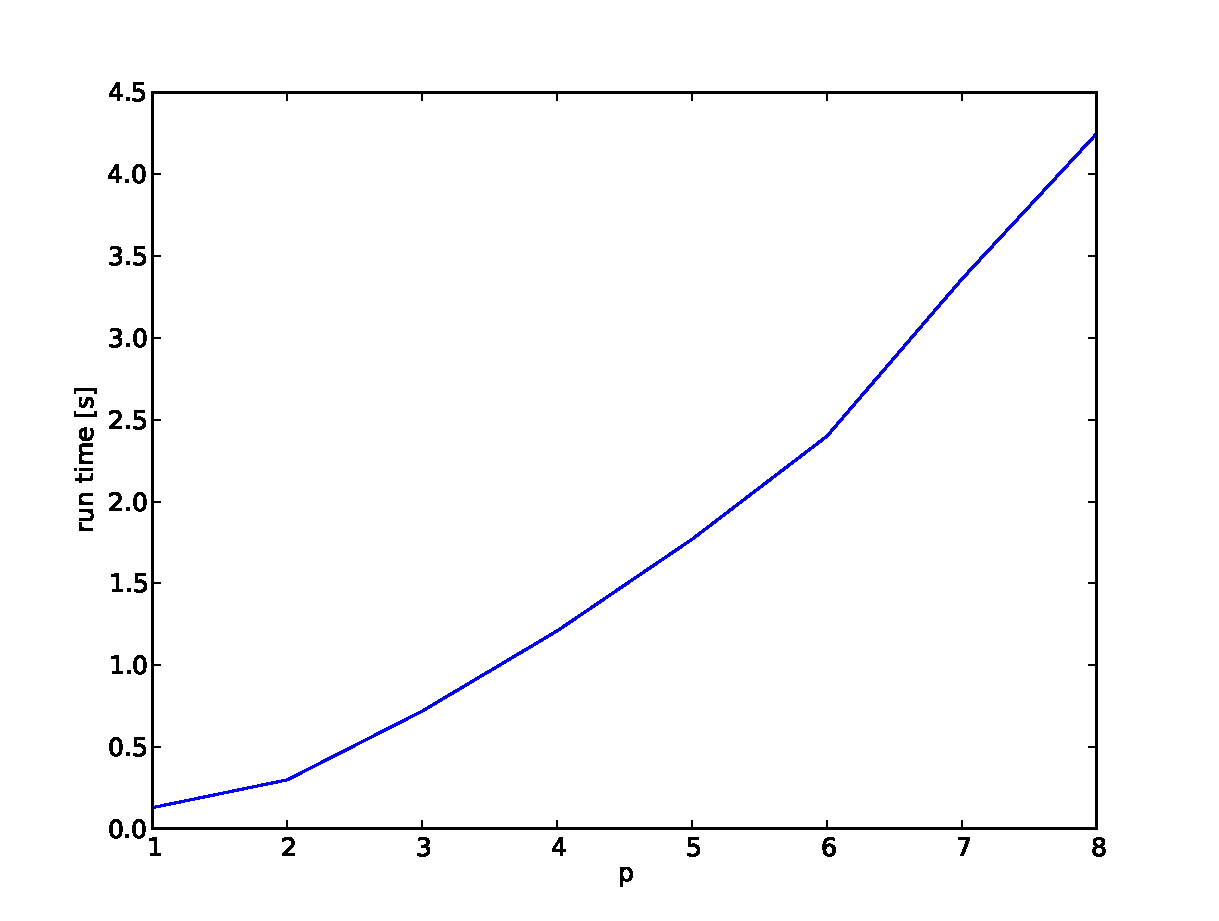
\includegraphics[width=0.6\textwidth]{Lp_complexity.pdf}
  \caption{Computation times for computing $\Lpnorm{10^{-7}\omega^3 +
      10^-3\omega^2 + 150\omega}$ 16384 times for $p=2,4,8$.}
  \label{fig:Lp-complexity}
\end{figure}

The value of $a$ that yielded the best result was $a=2$. The error
increased by more than 20\% when $a$ was increased to 4 or 8, and more
than tripled for $a=1$. This is reasonable, since a we want close
transitions to receive higher weights, but a too high $a$ would make
the weighted mean converge to the argmax function instead, taking only
a single training transition into account.

The modifier $\sigma$ for the standard deviation of the offset to the
sampled particles had a large impact on the error. The best value was
$0.2$, the maximum value, meaning the magnitude of the offset could be
roughly a fifth of the width of the populated region of the database
in each direction. This may be a bit surprising at first thought, but
one has to remember that the database used was artificially
generated. Even real data samples suffer selection bias if the
training data is not sampled from the model one intends to
learn.\footnote{As mentioned in the section ``Data Preparation'' of
  Encyclopedia of Machine
  Learning. \cite{EncyclopediaMachineLearning}} In this case, the
training data is not sampled from real data, and furthermore was
generated with settings guessed after inspection of whisker
videos. This means that the training data is probably a bad
representative of whisker dynamics, and a large $\sigma$ therefore
helps ``blur out'' the deficiencies of the training data.

Another note on the bias effect of the database is the size of the
time step. In the first runs performed on real data, the time scale of
the database was approximately two thirds that of the video. The
result was that the posture estimations were left behind when the
whiskers moved away, and the model instances frequently jumped between
whiskers in the video. In conclusion, the time scale is perhaps one of
the most important properties of the training data.

Finally, the value of the parameter $g$ that minimized $E$ was
$g=4$. The dependence of $E$ on $g$, however, is unclear and no real
conclusions can be drawn from the results. No qualitative behavior
can be seen in the $g$ direction of figure \ref{fig:Esg-maxerr-L2}. It
is also difficult to predict what values of $g$ should give a good
performance. A low $g$ would make clutter too important. A high $g$
amplifies high responses, but a high response does not necessarily
mean that the posture coincides well with the whisker it is intended
to track. For instance, in the test run on real video there was a
small, bright whisker above the top tracked whisker, which sometimes
gave a higher response than the latter.




% One can say that $a$ determines how local the weighted mean should
% be.



\section{Possible improvements}

Judging by the results of the run on real data, the following are the
greatest weaknesses of the testing implementation:\footnote{Excluding
  the fact that the database is probably not representative of whisker
  dynamics}

\begin{itemize}
\item The whisker model expects whisker roots to be stationary.
\item The response function\footnote{Including the chosen
    transformation $\phi$} is too simple.
\end{itemize}

A combination of these manifested clearly in the run on real
data. Because of the first, the whisker models had to be rooted inside
the snout, meaning no response at all could be collected in a radius
of a few pixels from the root. This means that the estimated posture
could emerge from the snout at multiple locations and get comparable
responses, which in turn means the model could sometimes find a better
match by switching to another whisker. This combined with the low
temporal resolution of the video - which sometimes makes it difficult
even for a human to notice a ``swap'' between whiskers - makes it
difficult for the tracker to keep the model tracking the same
whisker. We therefore draw the following conclusion.

\begin{quote}
  A good whisker model must account for movements of the whisker root
  along the surface of the snout.
\end{quote}

Here the ``root'' of the whisker refers to the point where the whisker
shaft emerges from the snout.

Other possible improvements include:

\begin{itemize}
\item Developing a statistically rigorous response function. The one
  used in this thesis is very simple, and only gives a rough estimate
  of the probability that a hypothesis matches a whisker in the image,
  as indicated by figure \ref{fig:response_real}. A better solution
  might be to create a classifier that estimates the probability of a
  pixel being part of a whisker as opposed to the probability of being
  a non-whisker pixel, and combine multiple visual cues.\footnote{As
    is common in computer vision, and also used by
    Sidenbladh. \cite{Hedvig}} This might also include motion and
  direction cues, and not only pure pixel cues. A direction cue could
  consider the directions of whiskers, making it easier to cancel
  noise caused when whiskers cross.

  One could also investigate if it is possible to combine the particle
  filter with the analysis developed by Voigts et
  al. \cite{UnsupervisedTracking} as it proved to be a powerful
  classifier even on its own.

\item Having the tracker manage all whiskers simultaneously, as
  opposed to independently in sequence as is used in this thesis. The
  tracker could then avoid mapping multiple whisker models to the same
  whisker in the image, and attempt a perfect bipartite matching
  between time steps. This could make the jumps between whiskers less
  frequent, or perhaps eliminate them altogether.

\end{itemize}

\section{Conclusions}

We conclude that probabilistic whisker tracking is feasible, and our
results on tracking real whiskers are even quite promising. Our simple
implementation manages to track real whiskers, though the tracking is
very unreliable and the posture estimations frequently jump between
whiskers. With more work, including better image analysis and a
database of real data, the performance could probably be vastly
increased, and eventually compete with the best solutions available
today.

% use the word dataset, training data, test data(generated) test
% data(real) [test set] mention bias

% analysis on the use of analytical solution for Lp which is norm on
% the function itself (seen as an inf-dimensional vector) instead of
% its parameters (which we tested and had som problems with)


% supervised learning (add in text and analysis)
%
% One cant just see the tracking by just trying one step at the time
% in the same way as the database "generated" since we must measure
% the tendency for the algorithm to break down after a while, althoug
% it could be a fast interesting measure that we easily could have
% runned to see short term effects of changing the parameters then
% going up to longer term effects.
%
% "A learning algorithm must interpolate appropriate predictions for
% regions of the instance space that are not included in the training
% data." - Encyclopedia (>model evaluation)


% Can a particlefilter overfit?(should this perhaps be in theory?)
